\documentclass[twocolumn]{article}
\usepackage{color}
\usepackage{cite}
\usepackage{draftwatermark}
\usepackage{multirow}
\usepackage{listings}
\usepackage{float}
\usepackage{amsfonts}
\usepackage{amssymb}
\usepackage{amsmath}
\usepackage{amsthm}
\usepackage{epsfig}
\usepackage{epstopdf}
\usepackage{titling}
\usepackage{url}
\usepackage{enumitem}
\usepackage{array}
\usepackage[utf8]{inputenc}
\usepackage[english]{babel}
\usepackage{tikz}
\usepackage{algorithm}
\usepackage[noend]{algpseudocode}
\usepackage{abstract}

\usetikzlibrary{shapes,arrows,positioning,patterns,through}
\SetWatermarkText{Preview}
\SetWatermarkScale{1}
\setlength\parskip{.5\baselineskip}

\definecolor{pagecolor}{rgb}{1,0.98,0.9}
\pagecolor{pagecolor}

\tikzset{
  dot node/.style={
    shape=circle,
    fill=white,
    draw,
    inner sep=+0pt,
    minimum size=+5mm
  },
  dotdot node/.style 2 args={
    dot node,
    label={[shape=circle,fill=black,outer sep=+0pt,inner sep=+0pt,minimum size=+3mm,name=ddd-#1,#2]center:}
  },
  arc style/.style={
    |<->|,
    shorten >=+-.5\pgflinewidth,
    shorten <=+-.5\pgflinewidth,
  }
}

\author{
  Ryan J. Kung \\ ryankung@ieee.org \\
}
\title{Rings: A peer-to-peer network for sovereign age}


\begin{document}
\twocolumn[
  \begin{@twocolumnfalse}
    \maketitle
    \begin{abstract}

      Rings Network is a decentralized peer-to-peer network that has built a more decentralized, anonymous and privacy-oriented data sovereignty network based on Chord computation. Rings Network is built with a communication layer based on WebAssembly, which allows it to run directly in the browser and connect directly between browsers via the webRTC protocol, further solving the problem of the modern Internet being controlled by centralized entities. Rings Network supports the use of elliptic curves as DIDs for proofs, and its stability is sufficient to support a large number of nodes and efficient lookups, making the connection and data exchange between sovereign entities more secure, efficient, and direct. This paper introduces the four-layer architecture of Rings Network and analyzes Rings Network from various aspects, including network, traffic, orderer, security, and shows the unlimited possibilities of Rings Network itself and as an application platform.

  ~\\
  ~\\
\end{abstract}
\end{@twocolumnfalse}
]
\section{Introduction and Motivation}

Centralized systems have long posed significant privacy and security risks to Internet users, as evidenced by numerous studies \cite{Kshetri2014, Kokkonen2018, G2016, tim}. The emergence of decentralized technologies has therefore attracted considerable interest as a means of mitigating these risks, while moving towards a "sovereign age" characterized by increased user control and data ownership.

The Rings Network represents a decentralized peer-to-peer alternative that aims to address these privacy and security challenges, offering a secure and private means of conducting online interactions. The objective of this paper is to introduce the Rings Network and demonstrate its potential for mitigating the risks posed by centralized systems, thus advancing the development of a sovereign age.

The technical specifications and architecture of the Rings Network will be thoroughly analyzed and its potential impact on personal privacy and the internet will be explored. These findings will contribute to the ongoing discussions about the future of the internet and the role of decentralized technologies in enhancing privacy, security, and control for users.

This paper aims to make a meaningful contribution to the discourse surrounding decentralized solutions such as the Rings network and their ability to advance towards a more secure, private and sovereign Internet.

\subsection{Browser Native}

The Rings Network is characterized as a browser native network, where all nodes have equal status and can run within a browser with full functionality. This configuration enables decentralized communication and data storage, as users can participate in the network without relying on centralized infrastructure.


An important aspect of the Rings Network is its communication layer, which is based on WebRTC\cite{webrtc-standard} and WebAssembly\cite{webassembly}. The use of these technologies supports browser-based peer-to-peer networking, bypassing the need for traffic to traverse a centralized infrastructure. This eliminates concerns such as centralized control over domain and DNS systems and censorship that exist in traditional web networks.


WebRTC, as a standard for real-time communication on the internet, offers a smooth user experience for the Rings Network. Meanwhile, WebAssembly, a low-level binary format for web-based applications, provides the necessary performance for the network. These technologies are widely supported by contemporary browsers, making the Rings Network accessible to a vast user base.

Moreover, the integration of WebRTC and WebAssembly allows for the development of decentralized applications on Rings Network. This opens up an array of possibilities for decentralized services, including secure file sharing and decentralized exchanges. The Rings Network is versatile, providing a platform for the development of a variety of decentralized applications rather than being limited to a specific use case.

\subsection{Proof Based DID}


Decentralized Identifiers (DIDs) are a form of decentralized digital identity that are proof-based and can be resolved into a DID document. The DID controller proves its control over the DID document using cryptographic algorithms.

  The Rings Network supports DID proofs using any cryptographic algorithm and enables better interaction between DID subjects through a lookup algorithm. DID subjects can refer to any entity, including people, data, services, or abstract entities. Rings Network allows the network to generate network DIDs using a wide range of elliptic curve algorithms. This flexibility in DID credentials improves compatibility with a variety of blockchain systems, including Ethereum\cite{Ethereum}, Bitcoin\cite{Bitcoin}, Aptos, and Solana\cite{Solana}.

Incorporating DID proofs into the Rings network facilitates the development of secure and trusted methods for identifying and authenticating network participants. This, in turn, promotes the establishment of secure and confidential communications and data exchange based on trusted relationships between parties.


\subsection{Lookup Protocol and Encryption}

The Rings Network leverages the Chord algorithm\cite{Chord} for its lookup protocol, which allows for the efficient and scalable mapping of network participants. The network is organized as a ring topology, where each node is linked to two other nodes, maximizing the functionality of the Chord algorithm for quick and effective participant lookup and location.

In conjunction with the lookup protocol, the Rings Network employs end-to-end encryption utilizing the ElGamal encryption scheme, ensuring privacy and security in the transmission of information between nodes. This implementation of ElGamal encryption\cite{ElGamalEncryption} opens up the possibility for various cryptographic techniques, such as secret sharing\cite{ssss} mechanisms, interactive zero-knowledge proofs\cite{zkp}, and the author-merlin protocol\cite{amp}, among others.

These lookup protocol and encryption capabilities provide a secure and efficient method of communication and data sharing in the Rings Network, surpassing the privacy and security offerings of traditional centralized networks.

\subsection{Data and Service Provision}

The Rings Network is particularly advantageous for data and service provisioning because of its anonymity and security properties. To enable the secure storage and exchange of sensitive information, the network uses a scheme of virtual Decentralized Identifiers (DIDs) to represent data and services. Virtual DIDs can also be referred to as resource IDs, but unlike resource IDs, they can refer not only to data, but also to a service, an email address, or a decentralized Web site.
These virtual DIDs are derived by a specific algorithm, such as a cryptographic hash function, and are denoted as $f(x) \rightarrow DID$, where $f(x)$ represents the algorithmic transformation.

The virtual DIDs are indexed and retrieved on the network using the same lookup protocol, using the Chord algorithm, as non-virtual DIDs. Unlike non-virtual DIDs, virtual DIDs do not have their own Decentralized Identifier proofs, but they do provide a secure and anonymous mechanism for storing and accessing data and services within the Rings network. This expands the possibilities for decentralized data storage and service delivery, including secure file sharing and decentralized data marketplaces.

\section{Related Work}
In the field of decentralized networks, Rings Network is not the sole option available. There are several other decentralized networks, such as Tor, GnuNet, Nym, and IPFS, that aim to provide users with privacy, security, and censorship resistance. In this section, we will undertake a comparative analysis of Rings Network with other peer-to-peer (P2P) networks.

In P2P networks, Distributed Hash Tables (DHTs\cite{DHT}) are commonly utilized. Many prominent decentralized networks, such as Edonkey\cite{Edonkey}, Ethereum\cite{Ethereum}, IPFS\cite{IPFS}, and Libp2p\cite{Libp2p}, have adopted the Kademlia\cite{Kademlia} algorithm as their DHT solution. Nevertheless, Rings Network employs the Chord protocol for P2P communication, offering an easier implementation for broadcasting and gossip messages in comparison to the Kademlia algorithm utilized by IPFS and Ethereum. This discrepancy in protocols accounts for the limitations in performance of IPFS and Ethereum in transmitting broadcast and gossip messages. To address this challenge, Ethereum has incorporated the ENR protocol, which stores node IP addresses within the DHT. While this enhancement improves the network's ability to transmit gossip messages, it also creates a direct threat to node privacy and security.

On the other hand, Rings Network belongs to the category of structured P2P networks, while Nym, Bitcoin, and BitTorrent networks are considered unstructured P2P networks. Structured P2P networks, such as Rings Network, have a well-defined topology and routing mechanism, while unstructured P2P networks rely on nodes to discover and connect with each other in a random manner. This structured architecture grants Rings Network a higher degree of scalability, efficiency, and robustness compared to unstructured P2P networks.

In terms of P2P communication protocols, the Chord protocol is employed by Rings Network, whereas IPFS and Ethereum utilize the Kademlia algorithm. The Chord protocol is significantly easier to implement for broadcasting and gossip messages than the Kademlia algorithm, which explains the limitations in performance for IPFS and Ethereum in these areas. To counteract this limitation, Ethereum has adopted the ENR\cite{ENR} protocol, though this solution creates a tradeoff between improved gossip capabilities and compromised node privacy and security.

In contrast, Tor network and Nym network are not structured P2P networks but rather relay networks that are decentralized but not P2P. This results in various security issues, such as spy attacks and man-in-the-middle attacks, which are circumvented by Rings Network through its structured P2P architecture.

Finally, it is worth noting that Rings Network is a browser-native P2P network, a unique feature that sets it apart from other existing network implementations. Rings Network can be executed on browsers, mobile devices, or PCs, thus making it a true P2P network that provides every individual with complete control over their data sovereignty.
\section{The Rings Network Architecture}
The Rings Network architecture is modeled after the well-established seven-layer structure of the TCP/IP reference model \cite{TCP_IP}. However, to accommodate its unique features and design goals, the Rings Network architecture is streamlined into five distinct layers.

\begin{itemize}[itemsep=2pt,topsep=0pt,parsep=0pt]
\item Runtime Layer: This layer constitutes the underlying technical infrastructure of the Rings Network, utilizing the WebAssembly (wasm) technology and wasm-bindgen to establish the framework.
\item Transport Layer: The transport layer implements secure, real-time communication between network nodes through the implementation of the WebRTC protocol.
\item Network Layer: The network layer employs the Chord algorithm to enable the distributed hash table (DHT) and decentralized identifier (DID) resolution functionalities.
\item Protocol Layer: This layer outlines the utilization of elliptic curve cryptography to generate DIDs, DID sessions, and virtual DIDs for secure data storage and the creation of sub-rings.
\item Application Layer: This layer caters to the needs of network developers, featuring two demonstration applications: Chatter and Dweb.
\end{itemize}
% \begin{figure}[htpb]
% \centering
% \begin{tikzpicture}[every node/.style={anchor=base,text depth=.5ex,text width=4cm, text centered}]
% \node (1) at (4.5,0) {\textbf{Physical Layer}};
% \node (2) at (4.5,0.7) {\textbf{Data Link Layer}};
% \node (3) at (4.5,1.4) {\textbf{Network Layer}};
% \node (4) at (4.5,2.1) {\textbf{Transport Layer}};
% \node (5) at (4.5,2.8) {\textbf{Session Layer}};
% \node (6) at (4.5,3.5) {\textbf{Presentation Layer}};
% \node (7) at (4.5,4.2) {\textbf{Application Layer}};

% \draw[] (1.south west) -- (1.south east) -- (1.north east) -- (1.north west) -- cycle;
%   \draw[] (2.south west) -- (2.south east) -- (2.north east) -- (2.north west) -- cycle;
%   \draw[] (3.south west) -- (3.south east) -- (3.north east) -- (3.north west) -- cycle;
%   \draw[] (4.south west) -- (4.south east) -- (4.north east) -- (4.north west) -- cycle;
%   \draw[] (5.south west) -- (5.south east) -- (5.north east) -- (5.north west) -- cycle;
%   \draw[] (6.south west) -- (6.south east) -- (6.north east) -- (6.north west) -- cycle;
%   \draw[] (7.south west) -- (7.south east) -- (7.north east) -- (7.north west) -- cycle;
% \end{tikzpicture}
% \caption{The TCP/IP OSI Model}
% \end{figure}

\begin{figure}[htbp]
\centering
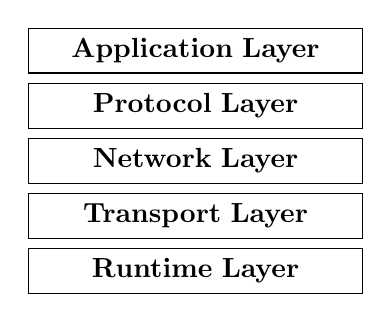
\begin{tikzpicture}[every node/.style={anchor=base,text depth=.5ex,text width=4cm, text centered}]
\node (1) at (4.5,0) {\textbf{Runtime Layer}};
\node (2) at (4.5,0.7) {\textbf{Transport Layer}};
\node (3) at (4.5,1.4) {\textbf{Network Layer}};
\node (4) at (4.5,2.1) {\textbf{Protocol Layer}};
\node (5) at (4.5,2.8) {\textbf{Application Layer}};

\draw[] (1.south west) -- (1.south east) -- (1.north east) -- (1.north west) -- cycle;
  \draw[] (2.south west) -- (2.south east) -- (2.north east) -- (2.north west) -- cycle;
  \draw[] (3.south west) -- (3.south east) -- (3.north east) -- (3.north west) -- cycle;
  \draw[] (4.south west) -- (4.south east) -- (4.north east) -- (4.north west) -- cycle;
  \draw[] (5.south west) -- (5.south east) -- (5.north east) -- (5.north west) -- cycle;
\end{tikzpicture}
\caption{Layers of Rings Network}
\end{figure}





\subsection{Runtime Layer}

The design goal of Rings Network is to enable nodes to run in any environment, including browsers, mobile devices, Linux, Mac, Windows, etc. To achieve this, we have adopted a cross platform compile approach to build the code. For non-browser environments, we use pure Rust implementation that is independent of any system APIs, making our native implementation system agnostic. For browser environments, we compile the pure Rust implementation to WebAssembly (Wasm) and use web-sys, js-sys, and wasm-bindgen to glue it together, making our nodes fully functional in the browser.


WebAssembly, or WASM, is a low-level binary format for executing code in web browsers. It provides a way for developers to write high-performance code in languages such as C, C++, and Rust, and then run that code in a browser with native performance. WebAssembly is designed to be fast and efficient, with a compact binary format that is easy to parse and execute. It uses a low-level instruction set, which makes it well-suited for demanding tasks such as cryptography, compression, and image processing.

\begin{figure}[htbp]
  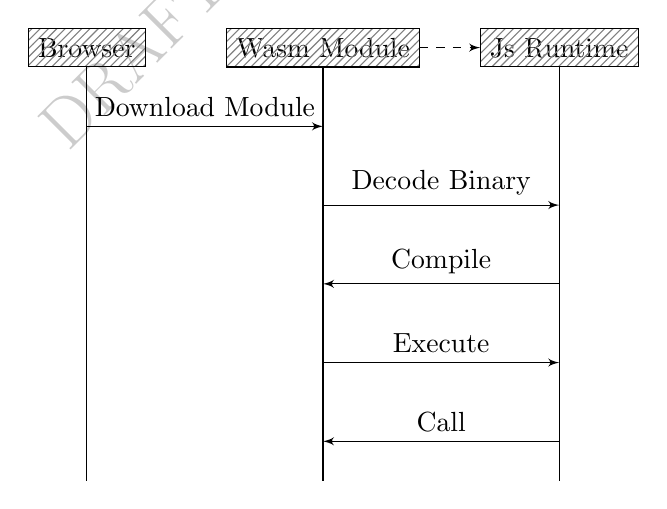
\begin{tikzpicture}[node distance=3cm,auto,>=latex']
  \node (A) {Browser};
  \node (B) [right of=A] {Wasm Module};
  \node (C) [right of=B] {Js Runtime};
  \draw (A) -- (A |-, -5.5);
  \draw (B) -- (B |-, -5.5);
  \draw (C) -- (C |-, -5.5);
  \draw[->] (A |-, -1) -- node[midway, above] {Download Module} (B |-, -1);
  \draw[->] (B |-, -2) -- node[midway, above] {Decode Binary} (C |-, -2);
  \draw[->] (C|-, -3) -- node[midway, above] {Compile} (B|-, -3);
  \draw[->] (B|-,-4) -- node[midway, above] {Execute} (C|-, -4);
  \draw[->] (C|-,-5) -- node[midway, above] {Call} (B|-,-5);
  \draw[pattern=north east lines, pattern color=gray] (A.south west) -- (A.south east) -- (A.north east) -- (A.north west) -- cycle;
  \draw[pattern=north east lines, pattern color=gray] (B.south west) -- (B.south east) -- (B.north east) -- (B.north west) -- cycle;
  \draw[pattern=north east lines, pattern color=gray] (C.south west) -- (C.south east) -- (C.north east) -- (C.north west) -- cycle;
  \draw[->,dashed] (B) -- (C);
\end{tikzpicture}
\caption{How WASM module works}
\end{figure}

The Rings Network provides multiple options for interacting with WebAssembly (WASM) modules, allowing developers to choose the method that best fits their needs.

1.\textbf{Building Rings Network applications and extensions using WASM-based frameworks}: This option provides the power and efficiency of developing applications with WebAssembly (WASM). Developers can leverage the performance and security benefits of WASM to build scalable and secure applications that run natively in the browser.
1. Building Rings Network applications and extensions using WASM-based frameworks such as Yew.

2.\textbf{Loading WASM modules through the exported JavaScript module}: This option is ideal for developers who prefer to work in JavaScript and want to take advantage of the benefits that WASM modules can offer. The Rings Network provides a JavaScript module that can be imported and utilized in other projects, allowing developers to easily load and utilize WASM modules within their own applications.

3.\textbf{Interacting with WASM modules through the Rings Network browser plugin}: The Rings Network browser plugin provides a convenient and accessible way for developers to interact with WASM modules. The plugin mounts the Rings Network provider to the "window.rings" object, allowing developers to interact with the Rings Network provider directly within their browser. This option provides a streamlined development experience, eliminating the need to navigate through multiple layers of code or configurations.
\subsection{Transport layer}
 The implementation of WebRTC and WebAssembly in Rings Network provides several advantages for users. Firstly, the browser-based approach means that users do not need to install any additional software or plugins to participate in the network. Secondly, the use of WebRTC and WebAssembly enables the network to have a low latency and high throughput, making it suitable for real-time communication and data transfer.

 WebRTC, or Web Real-Time Communication, provides browsers and mobile apps with real-time communication capabilities through simple APIs. With WebRTC, users can easily send audio, video, and data streams directly between browsers, without the need for any plug-ins or extra software.
At the same time, the Rings Network has some special optimizations for the WebRTC handshakes process.
 Assuming Node A and Node B want to create a WebRTC connection, they would need to exchange a minimum of three messages with each other:

 \begin{itemize}[itemsep=2pt,topsep=0pt,parsep=0pt]
  \item Node A gathers a list of ICE candidates and generates an SDP offer. The SDP offer includes information about the media streams and network addresses that Node A is willing to receive or transmit.
  \item Node A sends the SDP offer to Node B.
  \item Node B receives the SDP offer and starts gathering its own list of ICE candidates.
  \item Node B generates an SDP answer in response to the SDP offer received from Node A. The SDP answer includes information about the media streams and network addresses that Node B is willing to receive or transmit.
  \item Node B sends the SDP answer and its list of ICE candidates back to Node A.
  \item Node A receives the SDP answer and the list of ICE candidates from Node B.
  \item Node A and Node B use the ICE candidates and SDP information to establish a connection and establish a peer-to-peer communication channel.
  \end{itemize}

\begin{figure}[htbp]
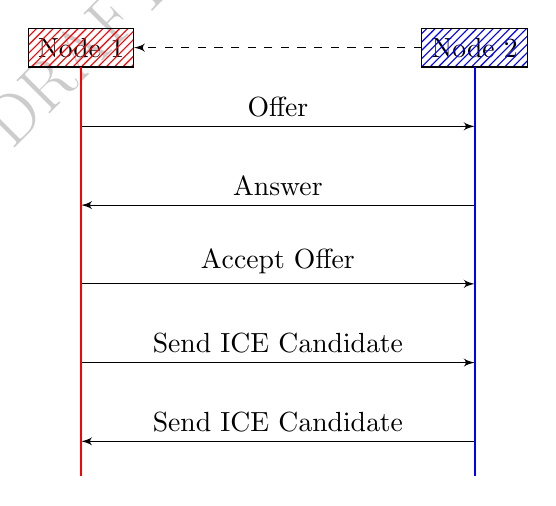
\begin{tikzpicture}[node distance=5cm,auto,>=latex']
  \node (A) {Node 1};
  \node (B) [right of=A] {Node 2};
  \draw[->] (A |-, -1) -- node[above] {Offer} (B |-, -1);
  \draw[->] (B |-, -2) -- node[above] {Answer} (A|-, -2 );
  \draw[->] (A |-, -3) -- node[above] {Accept Offer} (B |-, -3);
  \draw[->] (A |-, -4) -- node[above] {Send ICE Candidate} (B |-, -4);
  \draw[->] (B |-, -5) -- node[above] {Send ICE Candidate} (A |-, -5);
  \draw[->,dashed] (B) -- (A);
  \draw[pattern=north east lines, pattern color=red] (A.south west) -- (A.south east) -- (A.north east) -- (A.north west) -- cycle;
  \draw[pattern=north east lines, pattern color=blue] (B.south west) -- (B.south east) -- (B.north east) -- (B.north west) -- cycle;
  \draw[red, thick] (A.south) -- ++(0,-5.2cm);
  \draw[blue, thick] (B.south) -- ++(0,-5.2cm);
\end{tikzpicture}

\caption{Exchange SDP}
\end{figure}
By optimizing the WebRTC handshakes process, the Rings Network reduces the latency and overhead associated with establishing WebRTC connections. This results in a more efficient and reliable communication experience for users.

  \begin{itemize}[itemsep=2pt,topsep=0pt,parsep=0pt]

\item Gather ICE candidates and create an SDP offer, which is sent to the other party.
\item The recipient accepts the offer and generates an SDP answer, which is sent back along with its own list of ICE candidates.
\item At this point, the connection is established and the peer-to-peer communication channel is ready for use.
\end{itemize}
At its core, WebRTC is based on the exchange of Session Description Protocol (SDP) between browsers. The SDP is used to negotiate the communication settings and exchange cryptographic keys, allowing for secure communication between browsers. The process of exchanging SDP and establishing a secure connection is known as the WebRTC handshake.

In Rings Network, the WebRTC handshake is optimized by generating both the ICE Candidates and Offer simultaneously and exchanging them in a single Request-Response transaction. This significantly improves the efficiency of the handshake between nodes.

Once the WebRTC handshake is complete, browsers can send and receive data streams directly, with low latency and high bandwidth. This makes WebRTC ideal for real-time communication applications, such as video conferencing, online gaming, and live streaming.


\begin{figure}[htbp]
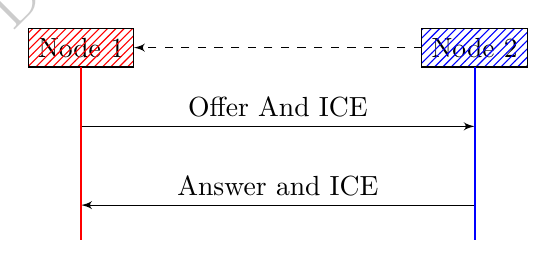
\begin{tikzpicture}[node distance=5cm,auto,>=latex']
  \node (A) {Node 1};
  \node (B) [right of=A] {Node 2};
  \draw[->] (A |-, -1) -- node[above] {Offer And ICE} (B |-, -1);
  \draw[->] (B |-, -2) -- node[above] {Answer and ICE} (A|-, -2 );
  \draw[->,dashed] (B) -- (A);
  \draw[pattern=north east lines, pattern color=red] (A.south west) -- (A.south east) -- (A.north east) -- (A.north west) -- cycle;
  \draw[pattern=north east lines, pattern color=blue] (B.south west) -- (B.south east) -- (B.north east) -- (B.north west) -- cycle;
  \draw[red, thick] (A.south) -- ++(0,-2.2cm);
  \draw[blue, thick] (B.south) -- ++(0,-2.2cm);
\end{tikzpicture}

\caption{Exchange SDP}
\end{figure}

\subsection{Network Layer}

The Rings Network is a structured peer-to-peer network that incorporates a distributed hash table (DHT) to facilitate efficient and scalable lookups. The Chord algorithm is utilized to implement the lookup function within the DHT, thereby enabling effective routing of messages and storage of key-value pairs in a peer-to-peer setting. The use of a DHT, incorporating the Chord algorithm, guarantees high availability in the Rings Network, which is critical for handling the substantial number of nodes and requests typically present in large-scale peer-to-peer networks.

Each node in the Rings Network is assigned a range of keys and maintains a finger table containing information about other nodes in the network. This allows for quick determination of the node responsible for a given key and facilitates the forwarding of queries to the appropriate node. The nodes and keys within the network are arranged in an identifier ring, which has at most $2^m$ nodes, ranging from 0 to $2^m-1$. The identifier ring provides a convenient method for mapping keys to nodes, and each node in the identifier ring has a successor and a predecessor. The successor of a node is the next node in the identifier ring in a clockwise direction, while the predecessor is the previous node in a counter-clockwise direction.

To maintain the robustness of the network in the event of node failures or departures, each node records a segment of the ring adjacent to it, including the preceding and following nodes. This results in a high probability that a node will be able to accurately locate its successor or predecessor, even in networks that experience a high failure rate. The information regarding the closest successor or predecessor of a node is stored in the finger table maintained by each node.

The Rings Network implements a more efficient search method to reduce query times and improve lookup efficiency. When a node seeks to look up a key, it forwards the query to the closest successor or predecessor of the key, as determined by the information stored in its finger table, until the key is found. This approach, similar to the approach employed by The algorithm, reduces the number of nodes that must be traversed to locate the responsible node, providing a scalable and efficient solution for data storage and retrieval within a peer-to-peer network.

In this way, the Chord algorithm provides a scalable and efficient way to store and retrieve data in a peer-to-peer network. The use of the hash function and finger table allow for efficient routing of queries and updates, while the decentralized nature of the network ensures high availability and robustness against node failures.

\begin{figure}[h]
    \begin{center}

  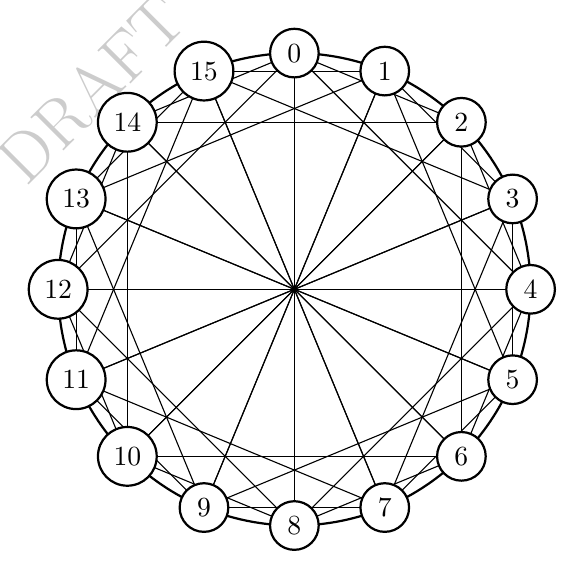
\begin{tikzpicture}[node distance=5cm,auto,>=latex']
    \xdef\N{16}
    \xdef\S{3}
    \xdef\deltadegree{360/\N}
    \draw[thick] (0,0) circle (\S);

    \foreach \i in {0,...,15} {
        % % predecessor
        % \pgfmathsetmacro{\result}{mod(\i-1,\N)}
        % \draw[color=red] (-\i*\deltadegree+90:\S) -- (-1*\result*\deltadegree+90:\S);

        % % successor
        % \pgfmathsetmacro{\result}{mod(\i+1,\N)}
        %     \draw (-\i*\deltadegree+90:\S) -- (-1*\result*\deltadegree+90:\S);

      % fingers
      \foreach \j in {1,...,4}{
            \pgfmathsetmacro{\result}{mod(\i+2^\j,\N)}
            \draw (-\i*\deltadegree+90:\S) -- (-1*\result*\deltadegree+90:\S);
        }
    }
    \foreach \i in {0,...,15}
    \node (\i) [circle,fill=white,draw=black,thick] at (-\i*\deltadegree+90:\S) {\i};
  \end{tikzpicture}
    \end{center}
    \label{dht}
      \caption{Chord algorithm, lookup protocol}

    \end{figure}
In the DHT, as illustrated in Figure \ref{dht}, all nodes have the capability to perceive their own predecessor and successor through the implementation of the join algorithm and stabilizationization algorithm. The predecessor of a node is determined as the node with the largest identifier that precedes the identifier of the current node in the identifier space. Conversely, the successor of a node is defined as the node with the smallest identifier that follows the identifier of the current node in the identifier space. These two nodes, the predecessor and the successor, are considered the immediate neighbor nodes of a particular node within the network.

\subsection{Protocol Layer}

In the protocol layer, the central design concept revolves around the utilization of a Decentralized Identifier (DID), which constitutes a finite ring in abstract algebra. The DID is a $2^{160}$-bit identifier that enables the construction of a mathematical structure that encompasses the characteristics of both a group and a field. It is comprised of a set of elements with two binary operations, addition and multiplication, which satisfy a set of axioms such as associativity, commutativity, and distributivity. The ring is deemed finite due to its having a finite number of elements. Finite rings are widely employed in various domains of mathematics and computer science, including cryptography and coding theory.

The properties of a finite ring in abstract algebra allow for the execution of addition and multiplication operations on the DID and for the comparison of their sizes. In certain cases, it can even be treated as a finite field, which expands the scope of cryptographic algorithms that can be utilized, such as the Secret Sharing Scheme (SSSS). The DID can be represented as $(R, +, \cdot, 0, 1, N)$, where $0$ represents the additive identity, $1$ represents the multiplicative identity, and "N" indicates that the ring has $2^{160}$ finite elements.

However, elements in an abstract algebraic structure of a finite ring cannot be directly subjected to greater than or less than operations. The BiasDID algorithm has been developed to address this limitation. The algorithm utilizes a fixed point to bias the DIDs within the ring, thereby ordering the elements in algebraic structures where direct greater than or less than operations are not feasible, but ordering is possible. In this manner, an element may always be to the right or left of another element, but it is closer to other elements. For instance, in the case of three elements, A, B, and C, they are ordered in a ring as A, B, C, A, B, etc. When treated as integers, A would always be greater than B and less than B. However, under the BiasDID algorithm, A is less than B since it is to the left of B, as determined through the comparison of the size of $A-C$ and $B-C$ using the fixed point C.


\begin{algorithm}[htpb]
\caption{Bias Order}
\label{alg:biasdid}
\textbf{Input}: Elements A and B, and fixed point C. \
\textbf{Output}: Result of comparison between A and B \
\begin{algorithmic}[1]
\State calculate $A-C$ and $B-C$
\If{$A-C < B-C$}
\State \textbf{return} $A < B$
\Else
\If{$A-C > B-C$}
\State \textbf{return} $B < A$
\Else
\State \textbf{return} $A = B$
\EndIf
\EndIf
\end{algorithmic}
\end{algorithm}


The DID, as an element of a finite ring, enables the computation of Virtual DIDs for data or message storage purposes. Virtual DID is another design of the protocol layer, which in principle can convert any data or service with any properties into a component of the network. This concept will be further elaborated in the subsequent sections.


The DID architecture also encompasses two critical modules, the Session and Message Relay. The former pertains to the generation of the DID and the utilization of existing elliptic curve algorithms and signatures of participants to establish and validate it. The latter describes the handling of messages, whether they be system messages or messages from a chat application.

\subsection{Application Layer}

The nucleus of Rings Network is similar to the Actor Model\cite{Actor_Model}, and it requires that each message type possess a Handler Trait. This allows for the separation of processing system messages, network messages, internal messages, and application-layer messages.

Rings Network provides a comprehensive set of interfaces for application-layer messages, which can be accessed through Remote Procedure Calls (RPC) or Foreign Function Interface (FFI). This implies that application developers have the option to not only control Rings Network through Rust or WebAssembly (Wasm), but can also access it via RPC using lighter weight programming languages such as Python or JavaScript. Furthermore, embedded developers can integrate Rings Network into microcontrollers through the use of FFI.

Additionally, applications can store data in the Distributed Hash Table (DHT) or register services, which depends on the credit of the participating nodes. This will be discussed in a subsequent chapter on the establishment of node credit.


\begin{figure}[htpb]
  \begin{center}
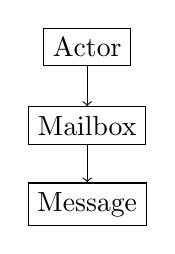
\begin{tikzpicture}
\node[rectangle, draw] (actor) {Actor};
\node[rectangle, draw, below of=actor] (mailbox) {Mailbox};
\node[rectangle, draw, below of=mailbox] (message) {Message};

\draw[->] (actor) -- (mailbox);
\draw[->] (mailbox) -- (message);
\end{tikzpicture}
\end{center}
\caption{Actor Model}

\end{figure}

Several demonstration applications have been implemented for the Rings Network, including a chat demo which allows users to communicate in a decentralized manner, and showcases the direct connection between browsers via handshaking. Another demo, similar to an onion network hidden service, enables anonymous access to services. There is also a DID demo referred to as BNS, which essentially serves as a pseudonymity service, issuing domain names and operable in conjunction with any blockchain.

\section{Algebraic Network}

In the Rings Network, DID is almost compatible with all elliptic curve algorithms, because we only need to use elliptic curve algorithms for DID proofs, which can be implemented through secp256k1, ed25519, or even RFID proof from hardware devices. We rely on external proofs to claim DID ownership in the Rings Network. In some simple cases, we can directly use the hash of the pubkey, such as secp256k1, which benefits from its signature recover algorithm. For ed25519, we use pubkey hash.

\subsection{Albegraic DID}

In Rings Network, the representation of Distributed Identifiers (DIDs) is achieved through the utilization of Finite Ring mathematics. The Finite Ring, not only serves as a ring-shaped topology in the network, but also as an abstract mathematical structure. The number of elements in this ring is represented by $2^{160}$, which is an astronomically large number, far surpassing the estimated number of ladders in the known universe. This results in the ring being sparse and discontinuous, and there is no direct relationship between $DID_n$ and $DID_{n+1}$. However, this mathematical structure allows us to place any data on the ring through the generation of appropriate Virtual DID (VID) values.

The calculation of DIDs within the Rings Network is performed in the context of the Finite Ring, including operations such as size comparisons and arithmetic operations like addition and subtraction. Additionally, the generation of VIDs for Channels or Data is also carried out using Finite Ring calculations. For example, the VID for a fixed participant group is calculated as the sum of the individual DIDs, while the VID for an unread Offline message is calculated as the recipient DID plus the message sequence number, both of which are elements in the finite ring. The DHT structure in Rings Network implements algorithms such as Join, Lookup, and stabilization, all of which are calculated within the confines of the finite ring.

\subsection{Network DID}

In a network topology, all the nodes form a ring structure and based on the Chord algorithm, we have implemented algorithms including join, lookup, and stabilization for the ring network.
\begin{algorithm}
\caption{DHT Join Algorithm}
\label{alg:join}
\begin{algorithmic}[1]
\Function{Join}{$n, node_id$}
\State $successor\gets find_successor(node_id)$
\State $predecessor\gets successor.predecessor$
\State $n.predecessor\gets predecessor$
\State $n.successor\gets successor$
\State $predecessor.successor\gets n$
\State $successor.predecessor\gets n$
\EndFunction
\end{algorithmic}
\end{algorithm}

When a participant joins the network, the node being joined will apply the Join algorithm, which will query a hashmap stored on each node, known as the Finger Table, and then determine whether it should be added to its own Finger Table. If not, the appropriate node is notified to construct a connection using the lookup algorithm.

The \textbf{join} algorithm ensures that all nodes in the network are aware of the new node's presence and are able to find it when necessary, allowing the network to remain scalable and consistent.

\begin{algorithm}[h]
\caption{DHT Lookup Algorithm}
\label{alg:lookup}
\begin{algorithmic}[1]
\Function{Lookup}{$key, node$}
    \State $finger\gets node.successor$
    \While{$finger.id \notin (node.id, key)$}
        \State $node\gets node.closestPrecedingNode(key)$
        \State $finger\gets node.successor$
    \EndWhile
    \State \Return $finger$
\EndFunction
\end{algorithmic}
\end{algorithm}



\begin{figure}[h]
      \begin{center}

  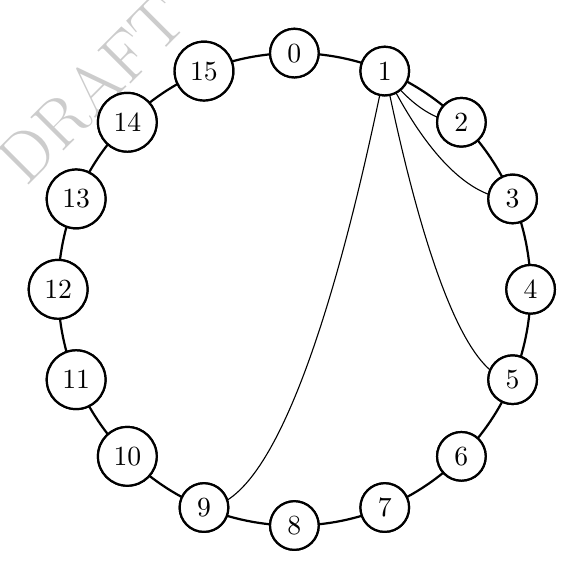
\begin{tikzpicture}[node distance=5cm,auto,>=latex']
    \xdef\N{16}
    \xdef\S{3}
    \xdef\deltadegree{360/\N}
    \draw[thick] (0,0) circle (\S);

    \foreach \i in {0,...,15} {
        % % predecessor
        % \pgfmathsetmacro{\result}{mod(\i-1,\N)}
        % \draw[color=red] (-\i*\deltadegree+90:\S) -- (-1*\result*\deltadegree+90:\S);

        % % successor
        % \pgfmathsetmacro{\result}{mod(\i+1,\N)}
        %     \draw (-\i*\deltadegree+90:\S) -- (-1*\result*\deltadegree+90:\S);

        % fingers
        % \foreach \j in {1,...,4}{
        %     \pgfmathsetmacro{\result}{mod(\i+2^\j,\N)}
        %     \draw (-\i*\deltadegree+90:\S) --- (-1*\result*\deltadegree+90:\S);
        % }
    }
    \foreach \i in {0,...,15}
    \node (\i) [circle,fill=white,draw=black,thick] at (-\i*\deltadegree+90:\S) {\i};
    \draw (1) parabola bend (2) (2);
    \draw (1) parabola bend (3) (3);
    \draw (1) parabola bend (5) (5);
    \draw (1) parabola bend (9) (9);
    \foreach \i in {0,...,15}
    \node (\i) [circle,fill=white,draw=black,thick] at (-\i*\deltadegree+90:\S) {\i};

  \end{tikzpicture}
      \end{center}

      \caption{Chord algorithm, lookup protocol}

    \end{figure}

The \textbf{lookup} algorithm from Chord is used to locate a specific node or data in a Chord-based distributed hash table network. The algorithm starts with the node making the lookup request, and it then follows the "fingers" in its Finger Table to determine which node is responsible for the data or node being searched for. If the responsible node is not the node making the lookup request, it forwards the request to the next node in its Finger Table until the responsible node is found. The algorithm is designed to be efficient and scalable, as it only requires $O(log N)$ hops to locate a node or data, where N is the number of nodes in the network. Additionally, the algorithm balances the load among the nodes in the network, ensuring that no single node becomes a bottleneck.

\begin{algorithm}[h]
\caption{DHT Stabilization}
\begin{algorithmic}[1]
\Procedure{Stabilize}{}
\State n.predecessor $\gets$ n.successor.predecessor
\If {$hash(n.predecessor) \in (hash(n), hash(n.successor)]$}
\State n.predecessor $\gets$ n.successor.predecessor
\EndIf
\State n.successor.notify(n)
\EndProcedure
\end{algorithmic}
\end{algorithm}

The \textbf{stabilization} algorithm is a process that runs periodically in a Chord network to ensure the consistency of the finger tables and the correct assignment of keys to nodes. The stabilization algorithm checks if a node's immediate successor is still its successor, and if not, it updates its successor to the node's current successor's successor. Additionally, the stabilize algorithm notifies the successor node that it is a potential predecessor. The aim of this process is to maintain the accuracy of the finger table and ensure that all nodes in the network have up-to-date information on the node responsible for a given key value. This helps to prevent key value assignment errors and reduces the number of lookups required to find the node responsible for a key, improving the efficiency of the network.

\subsection{Virtual DID}

In Rings Network, Virtual DID (VID) serves as a digital identifier that resembles a DID in format, but lacks the presence of DID Proofs within the limited scope of the network. Unlike physical computing nodes, VID manipulates the fingertable through algorithms such as lookup, stabilize, and application joining.

Various features within Rings Network, such as data storage, mailbox, sub-public channel, sub-ring, and hidden services, are all implemented through the use of VID. Data is mapped to a function H on the algebraic ring and stored within a distributed hash table (DHT), with different types of data assigned different Operators, including Overwrite, Extend, Touch, and JoinSubRing.

\textbf{Data storage} is the foundation for advanced data storage operations, and the Rings Network offers both Native and WASM implementations based on sled and indexDB, respectively. The storage capacity is up to 1G of local data. When a node is ready to store data, it generates a VID using the Hashing function H(D), and sends the data to its successor. The network will then locate the closest node or nodes to the data's VID using the lookup algorithm, depending on the number of replicas set.

In cases where the data is too large, it will be divided into chunks and assigned individual VIDs, which are stored independently on the network. The data's VID serves as a reference to these chunk VIDs. The lookup algorithm can be utilized to query and extend VIDs, as demonstrated by the implementation of the MailBox feature.

The \textbf{MailBox} provides a more anonymous communication channel, implemented for each DID by generating a VID using the rule $H("mailto") + DID$. The DID can retrieve messages from the MailBox through DID Proofs even when offline, eliminating the need for direct interaction with other nodes. Messages sent to the MailBox are encrypted using the public key associated with the DID through the Elgaml algorithm, ensuring that only the holder of the DID Proofs can access the message's content.

\textbf{Sub Ring} is a special kind of Data that is a minimized implementation of FingerTable but supports all algorithms that can be applied to Finger, including the join operator and lookup derivation. Sub Ring generates its VID through its name, with a very simple algorithm H(name). Sub Ring has its own MailBox on DHT to receive messages from Main Ring, and any member can choose to join Sub Ring, which will update the fingertable stored on Sub Ring using the join algorithm, while Sub Ring members will also keep their own copy of the finger table. It is important to note that the Finger table data stored on DHT and the Finger table data of Sub Ring participants are different, as their join algorithm and lookup algorithm have different fixed points on the finite Ring. For all DIDs, its fixed point is the DID itself.

\section{Traffic}

In Rings Network, the abstraction of traffic is divided into two approaches: Hop-by-Hop and End-to-End. Hop-by-Hop refers to a communication architecture where data is transmitted from one device to another through multiple intermediate systems in between. On the other hand, End-to-End (E2E) refers to a communication architecture where data is transmitted directly from the sender's device to the recipient's device without passing through any intermediate systems.


\subsection{Hop by Hop}

In Rings Network, a structured peer-to-peer network, we generate DID and DID proofs using widely used signature algorithms such as ECDSA or Ed25519. Then, we generate sessions for permission control based on the DID proofs. Our sessions are generated based on ECDSA, and can be seen as delegated private keys of the DID proofs' private keys. This is done to minimize the exposure of the original private keys and improve network security.

In order to better ensure message delivery and improve network stability, Rings Network implements its own MSRP based on the IETF draft. It is based on the Session system described above and the message types include Send and Report. It also caches the DID Path of the messages, which does not expose privacy and greatly enhances network robustness.

\subsection{End to End}

Rings Network places significant emphasis on End-to-End Encryption as a means to ensure privacy and security. Two main end-to-end encryption algorithms are used: RSA and Elgamal. RSA is typically used for lighter encryption needs while Elgamal is utilized for homomorphic encryption and other specialized scenarios.

Given an Elliptic curve cyclic group $\mathbb{G}$, of order $𝑞$ with generator $𝑔$. For private key $x, x\in\mathbb{Z}_q$, the public key is $g^x$. The curve can be secp256k1, ed25519, or other effeicent curves. We describe ElGamal encrypt and decrypt algorithm as below:

\begin{algorithm}[h]
\caption{ElGamal Encryption Algorithm}
\label{ElGamal Encryption}
\begin{algorithmic}[1]
\State \textbf{Input:} Message $m$, private key $x \in \mathbb{Z}_q$, public key $h = g^x$, generator $g$
\State \textbf{Output:} Encrypted message $(c_1, c_2)$
\Procedure{Encryption}{}
\State Choose a random integer $k \in \mathbb{Z}_q$
\State Compute $c_1 = g^k$
\State Compute $c_2 = m\cdot h^k$
\State \Return $(c_1, c_2)$
\EndProcedure
\Procedure{Decryption}{}
\State Compute $m = c_2\cdot(c_1)^{-x}$
\State \Return $m$
\EndProcedure
\end{algorithmic}
\end{algorithm}

\begin{algorithm}[htpb]
\caption{ElGamal Decryption Algorithm}
\label{ElGamal Decryption}
\begin{algorithmic}[1]
\State \textbf{Input:} Encrypted message $(c_1, c_2)$, private key $x \in \mathbb{Z}_q$
\State \textbf{Output:} Decrypted message $m$
\Procedure{Decryption}{}
\State Compute $m = c_2\cdot(c_1)^{-x}$
\State \Return $m$
\EndProcedure
\end{algorithmic}
\end{algorithm}


The advantage of the ElGamal algorithm is that it is a homomorphic encryption algorithm. This means that it allows mathematical operations to be performed on the ciphertext, and the result of the operations will be equivalent to the operations performed on the plaintext. This property makes ElGamal useful in various cryptographic applications, such as secure multi-party computation, where multiple parties can perform computations on encrypted data without exposing the plaintext.

The ElGamal encryption algorithm can be used to implement a secret sharing scheme (SSSS), where a secret is divided into multiple shares that are distributed among multiple participants. The secret can only be reconstructed if a sufficient number of shares are combined. In this scheme, the secret is encrypted under the public key of each participant using ElGamal encryption, and the resulting ciphertexts are used as shares. Decryption requires a sufficient number of participants to combine their shares and perform the decryption process using their private keys. Because ElGamal is a public-key encryption algorithm, this approach ensures that each participant's share remains confidential, as it can only be decrypted by the corresponding private key. This makes ElGamal a useful tool for implementing secure secret sharing schemes.


\begin{algorithm}[h]
\caption{ElGamal Secret Sharing Scheme}
\label{ElGamal SSSS}
\begin{algorithmic}[1]
\State \textbf{Input:} Secret $s$, public key $h = g^x$, generator $g$, number of shares $n$, minimum number of shares required to reconstruct the secret $k$
\State \textbf{Output:} $n$ shares $(c_{1,1}, c_{1,2}), (c_{2,1}, c_{2,2}), \dots, (c_{n,1}, c_{n,2})$
\Procedure{Encrypt}{}
\For{$i = 1$ to $n$}
\State Choose a random integer $r_i \in \mathbb{Z}q$
\State Compute $c{i,1} = g^{r_i}$
\State Compute $c_{i,2} = s\cdot h^{r_i}$
\EndFor
\State \Return $(c_{1,1}, c_{1,2}), (c_{2,1}, c_{2,2}), \dots, (c_{n,1}, c_{n,2})$
\EndProcedure
\Procedure{Decrypt}{}
\State Choose $k$ shares $(c_{i_1,1}, c_{i_1,2}), (c_{i_2,1}, c_{i_2,2}), \dots, (c_{i_k,1}, c_{i_k,2})$
\State Compute $s = \prod\limits_{j=1}^k c_{i_j,2} \cdot \left(\prod\limits_{j=1}^k c_{i_j,1}\right)^{-x}$
\State \Return $s$
\EndProcedure
\end{algorithmic}
\end{algorithm}


\begin{algorithm}
  \caption{SSSS over a finite ring}
  \label{FR SSSS}
\begin{algorithmic}[1]
\Procedure{SSSS}{$s$, $p$, $g$, $t$, $n$}
\State Choose a prime number $p$ and a primitive element $g$ in the ring $\mathbb{Z}_p$
\State Define a polynomial $f(x) = s + a_1 x + a_2 x^2 + \cdots + a_{t-1} x^{t-1}$ of degree $t-1$
\For{$i = 1, 2, \ldots, n$}
\State Compute $s_i = f(g^i) = s + a_1 g^i + a_2 (g^i)^2 + \cdots + a_{t-1} (g^i)^{t-1}$
\EndFor
\State \Return $(s_1, s_2, \ldots, s_n)$
\EndProcedure
\end{algorithmic}
\end{algorithm}



 Algorithm \ref{ElGamal SSSS} serves as an exemplification of the utilization of the ElGamal algorithm to realize Secret Sharing Schemes (SSSS). Given the fact that the Distributed IDs (DIDs) on the Chord Distributed Hash Table (DHT) form a finite ring, it is feasible to directly implement SSSS by leveraging this characteristic. By executing the SSSS protocol over the Chord DHT, the confidentiality and security of the secret is ensured through its decentralized distribution and storage. Each node within the DHT only assumes responsibility for retaining its respective share, which remains encrypted and can only be accessed through the usage of its corresponding private key. This attributes the Chord DHT with a superior suitability as a platform for implementing secure SSSS. The algorithm for implementing a Secret Sharing Scheme (SSSS) over a finite ring can be represented as lgorithm \ref{FR SSSS}

 \subsection{Chunking}

 When the size of the message to be transferred exceeds the maximum transmission unit (MTU) of the transport layer, chunking is employed to divide the data into smaller parts, and each part is transmitted in a smaller packet. This reduces the strain on the network and increases the probability of successful data transfer. There are two implementations of chunking, end-to-end and hop-by-hop. End-to-end chunking involves directly sending chunks through one or multiple successors for each request, and the receiver takes responsibility for reassembling and ordering the chunks as well as requesting retransmission when needed. Hop-by-hop chunking, on the other hand, takes place at the transport layer and offers a more robust way to transmit data, but its efficiency may be lower due to the varying MTU of nodes. However, this implementation is usually more reliable.

 \begin{algorithm}[h]
\caption{End-to-End Chunking Algorithm}
\label{alg:e2e_chunking}
\begin{algorithmic}[1]
\Procedure{E2E Chunking}{}
\State Input: data, chunk size
\State Output: chunks
\State chunks $\gets$ []
\State total-chunks $\gets$ ceil(len(data)/chunk-size)
\For{i in range(total-chunks)}
\State chunk $\gets$ data[i*chunk-size : (i+1)*chunk-size]
\State append chunk to chunks
\EndFor
\State \Return chunks
\EndProcedure
\end{algorithmic}
\end{algorithm}

Algorithm \ref{alg:e2e_chunking} shows how a common chunking algorithm works. In this algorithm, the input data is divided into a number of chunks equal to the ceiling of the length of the data divided by the chunk size. For each iteration of the loop, a chunk of the specified size is extracted from the data and added to the list of chunks. The list of chunks is then returned as the output of the algorithm.

\section{The Orderer}

An orderer in a distributed system is a component responsible for determining the order in which messages are delivered or transactions are executed. In other words, the orderer ensures that events in the system occur in a predictable and consistent order, even when they originate from different sources. This is important for maintaining the integrity and consistency of the system and avoiding conflicts or inconsistencies.

Lamport described the order of messages as a result of time-stamping each message that is sent between nodes in a distributed system. This involves assigning a unique logical timestamp to each message, which represents the logical order in which the messages were generated. The timestamps are used to determine the order in which the messages should be processed, so that the recipient node can ensure that messages are processed in a consistent and reliable manner, regardless of the order in which they were actually received.

\subsection{Sidecar Orderer}

Lamport timestamps, as outlined in Algorithm \ref{lamport ts}, can facilitate simple message ordering in distributed systems. However, it is not secure and can be prone to attacks. Hence, the Sidecar Orderer mechanism is introduced as a more secure alternative.

\begin{algorithm}[h]
\caption{Lamport timestamp}
\label{lamport ts}
\begin{algorithmic}[1]
\State Initialize local time $localTime \gets 0$
\State On sending message $m$:
\State \quad $localTime \gets localTime + 1$
\State \quad Set $timestamp(m) = localTime$
\State On receiving message $m$:
\State \quad $localTime \gets \max(localTime, timestamp(m)) + 1$
\end{algorithmic}
\end{algorithm}


In a distributed system, the Sidecar Orderer operates as an external entity, not integrated into the system itself. Instead of relying on an internal formal algorithm for ordering, the system utilizes an external witness to establish message ordering.
In the context of Rings Network, message ordering is achieved through the utilization of a Sidecar Orderer. This can be a blockchain technology such as Ethereum, Bitcoin, or any other. Messages requiring a determined order must prove, through the time-stamping capabilities of the blockchain, that their transmission time was not earlier than a specified timestamp.
As a validator, Rings Network supports the ordering of messages from different sources. For instance, Message A employs the hash $\sigma$ of a Bitcoin block to demonstrate that its time is not later than $t_a$, while Message B utilizes the hash $\beta$ of a Solana block to prove that its time is not later than $t_b$. Given that $t_a < t_b$, Message A precedes Message B.

However, the Sidecar Orderer is limited in its capabilities as it can only provide proof of the latest possible time for a message. For instance, when Message A asserts time $t0$, it can only demonstrate that its transmission time is not before $t0$, thus constituting a proof of the latest time. Additionally, the varying granularity of proofs from different witnesses often results in a partial order of messages, which may temporarily result in parallel timelines.


\subsection{Byzantine fault tolerance}
Although Rings Network supports Sidecar Orderer, it does not aim to achieve Byzantine Fault Tolerance (BFT). This is because the implementation of the Rings Network Orderer relies on an external BFT, which means that it can run smoothly without the need for implementing its own consensus system. The use of an external BFT allows Rings Network to focus on other aspects of its design, without the need for in-depth expertise in consensus algorithms. This also means that Rings Network can take advantage of the security and robustness of existing BFT systems, which have been widely tested and proven in various applications. As a result, Rings Network can provide a secure and efficient solution for message ordering in distributed systems without having to deal with the complex problems of consensus algorithms.

\subsection{Ranking Protocol}


The proposed ranking protocol aims to provide a fair and accurate evaluation of nodes within a distributed network. The system operates by having nodes rank each other based on a set of predefined criteria, such as availability, response time, and data transfer speed.


\begin{algorithm}[h]
\caption{Ranking Protocol Algorithm}
\label{alg:ranking-protocol}
\begin{algorithmic}[1]
\Procedure{Rank}{$N$, $nodes$}
\State $rankings$ $\gets$ $\emptyset$
\For{$i \gets 1$ to $N$}
    \State randomly sample a node $j$ from $nodes$
    \State $nodeRankings$ $\gets$ getRankings($j$)
    \State $rankings$.add($nodeRankings$)
\EndFor
\For{$node \in nodes$}
    \State $medianScore$ $\gets$ calculateMedianScore($rankings$, $node$)
    \State $node$.setScore($medianScore$)
\EndFor
\EndProcedure
\Procedure{GetRankings}{$node$}
\State $rankings$ $\gets$ $\emptyset$
\For{$otherNode \in nodes$}
    \State $rank$ $\gets$ $node$.rank($otherNode$)
    \State $rankings$.add($rank$)
\EndFor
\State \Return $rankings$
\EndProcedure
\Procedure{CalculateMedianScore}{$rankings$, $node$}
\State $medianScore$ $\gets$ median of all $rankings$ for $node$
\State \Return $medianScore$
\EndProcedure
\end{algorithmic}
\end{algorithm}

To ensure that the rankings are representative of the network, a random sampling approach is employed. By using a random number generator or random oracle, the sampling of nodes is performed in a truly random fashion. The collected rankings are then subjected to a median calculation to mitigate the impact of outliers. To further enhance the accuracy of the rankings, the collected rankings can be weighted based on the rank token of the node that provided the ranking.

To prevent malicious nodes from providing false rankings, the ranking protocol implements a proof-of-ranking mechanism. This requires nodes to provide proof of their rankings, such as by signing the random seed used in the sampling and the rankings of other nodes. Additionally, a punishment mechanism is implemented to penalize nodes that misbehave, such as by reducing their ranking score or rewarding other nodes for reporting the misbehavior.

In order to prevent Sybil attacks, the ranking protocol considers a freeze period. After a node claims its ranking score, its tokens are frozen for a certain period to prevent it from claiming multiple rankings. This protects the integrity of the ranking system and ensures that it accurately reflects the behavior of nodes within the network.

The ranking score of a node $i$ is represented by $r_i$. The rankings of a node $i$ for other nodes in the network are represented by $R_{i,j}$, where $j$ is the index of another node in the network. The median score of a node $i$ is represented by $m_i$, which is calculated as:

\begin{gather}
m_i = \text{median}(R_{i,j})
\end{gather}

The weight of a ranking provided by a node $i$ is represented by $w_i$, which is based on the rank token of node $i$. The weighted median score of a node $i$ is represented by $w_{m_i}$,, which is calculated as:

\begin{gather}
w_{m_i} = \text{median}(w_i \cdot R_{i,j})
\end{gather}

\section{Performance}

We will discuss the performance of Rings Network from two aspects: Latency, Reliability.

\subsection{Latency}
For Rings Network, latency mainly comes from the lookup/routing process of the Chord algorithm. During this process, some redirects may occur due to the influence of network instability. In the simulator of the Chord algorithm, we can find that when the failure rate of the network is 50\%, the average number of hops in the lookup will reach about 5 on average. We consider this level of latency to be acceptable.

\begin{table}[htbp]
\begin{tabular}{l|l|l}
\cline{1-3}
  \shortstack{Fraction of \\failed nodes} & \shortstack{Mean \\routing hops} &\shortstack{Mean num. of \\lookup timeouts}   \\ \cline{1-3}
0                        & 3.84             & 0.0                     \\ \cline{1-3}
0.1                      & 4.03             & 0.60                    \\ \cline{1-3}
0.2                      & 4.22             & 1.17                    \\ \cline{1-3}
\end{tabular}
\caption{Latency on failed node rate of Chord \cite{Chord}}
\end{table}

\begin{figure*}[htbp]
  \label{path}
  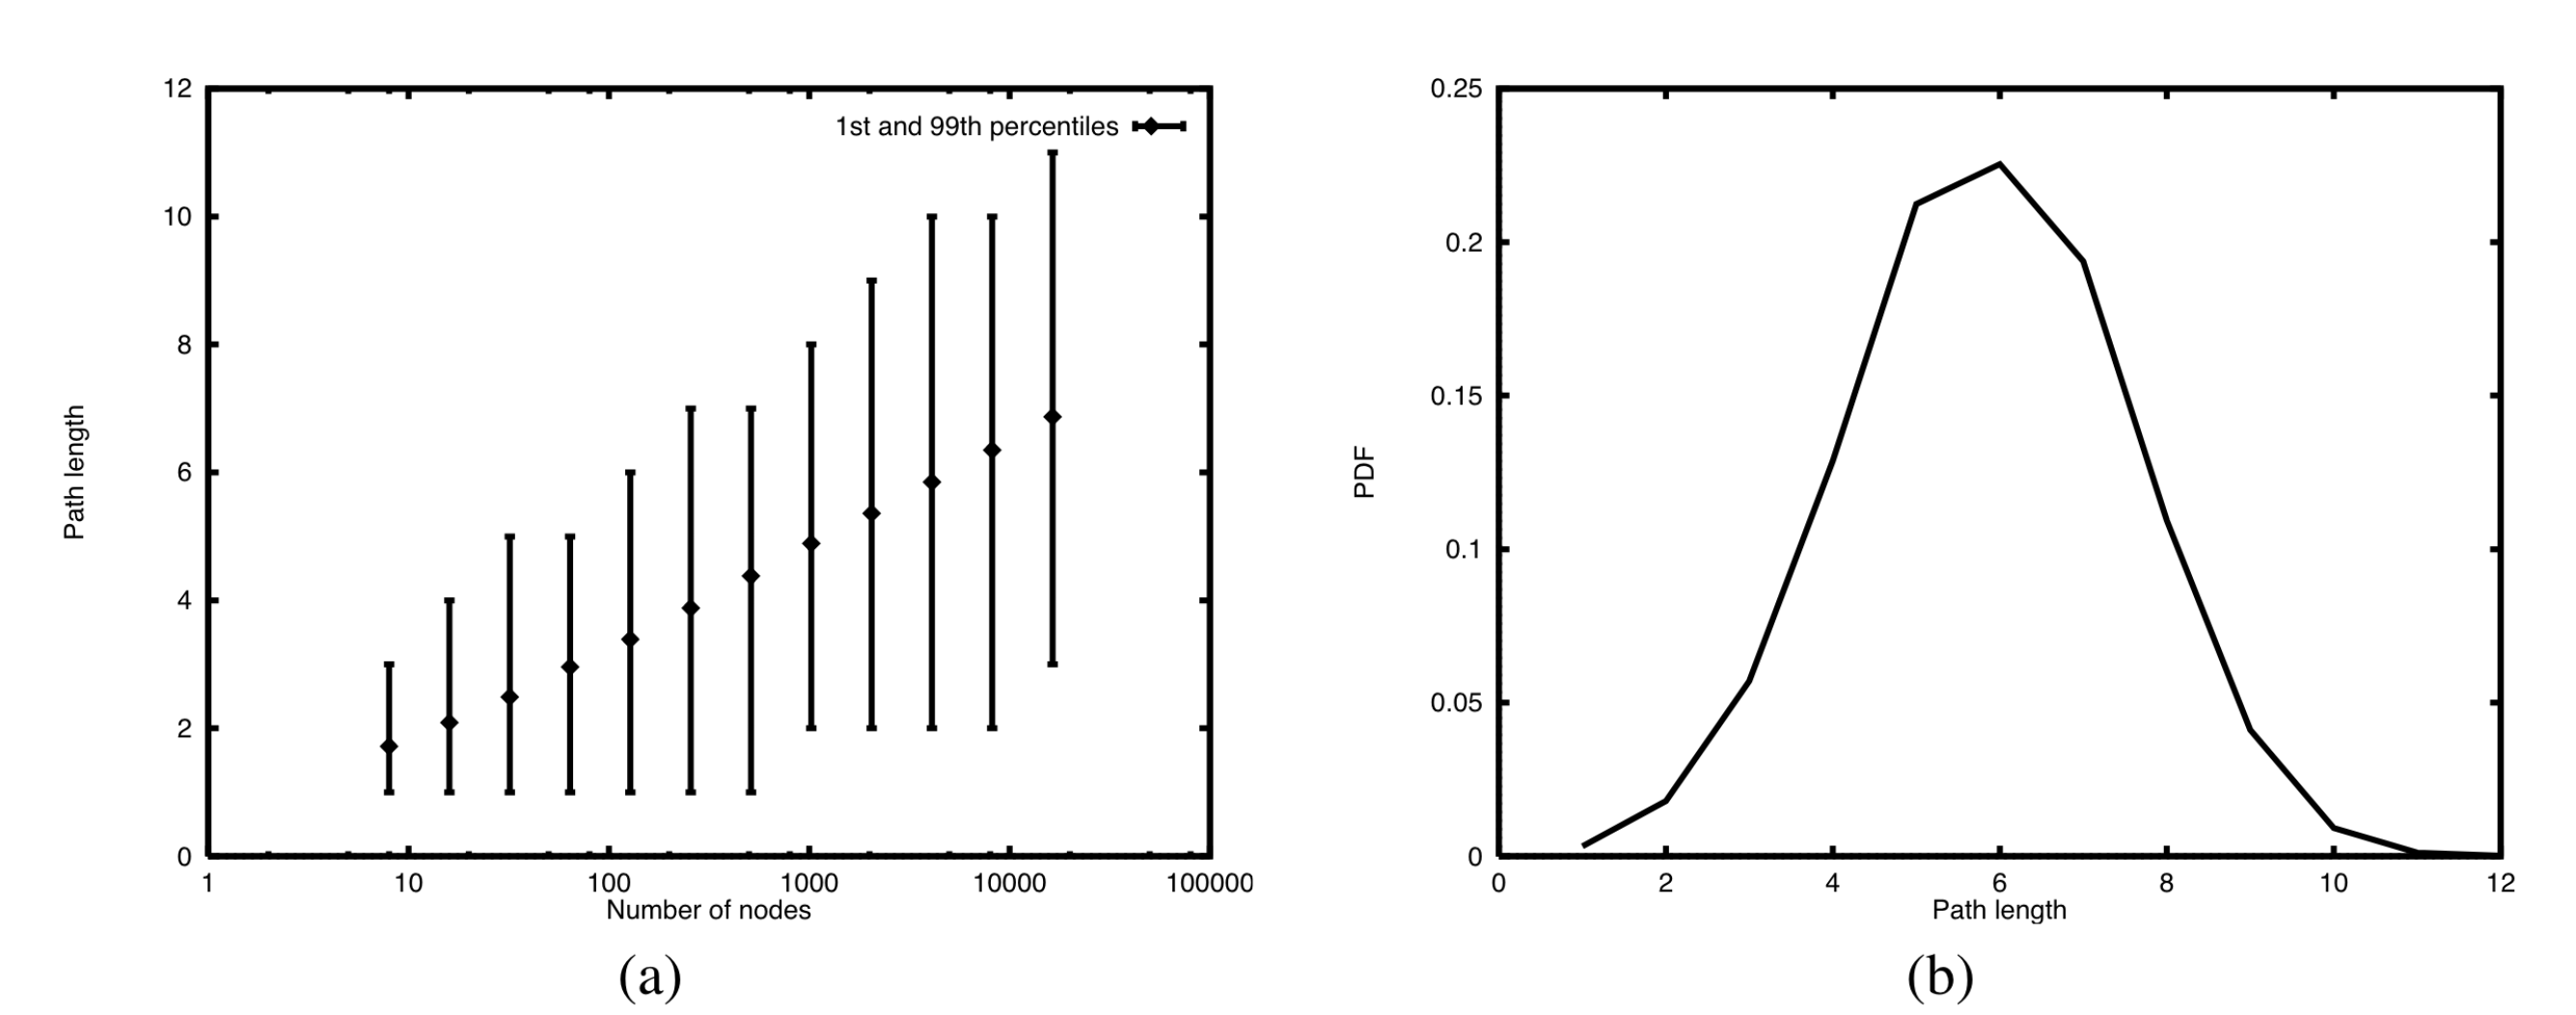
\includegraphics[width=\linewidth]{imgs/rings/path.png}
  \caption{Chord lookup path \cite{Chord}}
\end{figure*}

According to the simulation results, when the number of nodes increases from 10 to 100K, the path length only increases by about 3 times. The left side of Figure \ref{path} shows this scenario, and the right side is the PDF (probability density function) of the path length.
\subsection{Reliablility}

Rings Network allows full node functionality in browsers, enabling nodes to easily connect with each other. However, this also increases their join/leave rate. Hence, the network's performance with frequent node join/leave events is crucial for evaluation.

\begin{table}[htpb]

    \label{failure}
  \begin{tabular}{l|l|l|l}
\cline{1-4}
  \shortstack{join/leave rate \\ (per sec./stab. \\ period)}
  & \shortstack{Mean \\routing\\ hops}
  &\shortstack{Mean \\num. of \\lookup \\timeouts}
  &\shortstack{Lookup \\ failures \\ per 10k} \\ \cline{1-4}
0.05/1.5                        & 3.90             & 0.5              &    0   \\ \cline{1-4}
0.10/2                      & 3.83             & 0.11             &    0   \\ \cline{1-4}
  0.15/4.5                      & 3.84             & 0.16             &    2   \\ \cline{1-4}

  0.20/6                      & 3.81             & 0.23             &    5   \\ \cline{1-4}
0.25/7.5                      & 3.83             & 0.30             &    6   \\ \cline{1-4}
  0.30/9                      & 3.91             & 0.34             &    8   \\ \cline{1-4}
  0.35/10.5                      & 3.94             & 0.42             &    16   \\ \cline{1-4}
0.40/12                      & 4.06             & 0.46             &    15   \\ \cline{1-4}

\end{tabular}
\caption{Failure rate of Chord \cite{Chord}}
\end{table}

Figure \ref{failure} shows that in simulation, as the network's join/leave rate increases from 5\% to 40\%, the availability of the network reaches 99.85\% even under the worst conditions (join/leave rate of 40\% per second).


\section{Security}
As a decentralized platform, Rings Network is susceptible to various security risks and malicious attacks. Therefore, it is crucial to implement robust security measures to ensure the integrity and confidentiality of the network.
\begin{itemize}[itemsep=2pt,topsep=0pt,parsep=0pt]
\item Sybil Attack: A Sybil attack represents a malicious attempt to undermine the trust and control of a network by creating multiple fake identities. To counter this threat, Rings Network implements the Ranking protocol, which enhances network security through local and global ranking mechanisms. New nodes, which possess a low ranking rate, find it challenging to swiftly earn the credibility of neighboring nodes, thereby deterring Sybil attacks.

\item Replay Attack:
  A replay attack constitutes a malicious attempt to disrupt a network by intercepting and retransmitting a legitimate network transmission. To counteract such threats, Rings Network employs digital signatures and cryptographic hashes to guarantee the authenticity of messages and prevent their repeat usage. Additionally, the Sidecar Orderer serves as an indispensable and dependable tool for ordering critical non-replayable messages in Rings Network.

\item Man-in-the-Middle Attack:
  A man-in-the-middle (MITM) attack represents a malicious attempt to intercept and potentially modify or eavesdrop on communication between two parties. To prevent such attacks in Rings Network, the validation of elliptic curve signatures and the implementation of end-to-end encryption render such attacks entirely infeasible.

\item Denial of Service Attack
A denial-of-service (DoS) attack is a type of cyberattack where an attacker sends a large volume of requests to a network to overwhelm it and disrupt its normal functioning. In Rings Network, the implementation of rate limiting mechanisms and ranking protocol can help to prevent DoS attacks and ensure the stability of the network.
\end{itemize}

\section{Conclusion}
The Rings Network is a decentralized, peer-to-peer network architecture optimized for the digital era of sovereignty. It offers a secure and efficient solution for communication, data storage, and service delivery, by leveraging cutting-edge technologies such as WebRTC, WebAssembly, and decentralized identifier (DID) proofs, along with a lookup protocol and encryption scheme. Additionally, its support for virtual DIDs makes the Rings Network a paradigm-shifting solution in the realm of decentralized networks and applications.

\bibliographystyle{unsrt}
\bibliography{./cites}
\end{document}